\documentclass{article}
\usepackage{listings}
\usepackage{mathrsfs}
\usepackage[utf8]{inputenc}
\usepackage{amssymb}
\usepackage{lipsum}
\usepackage{amsmath}
\usepackage{fancyhdr}
\usepackage{geometry}
\usepackage{scrextend}
\usepackage[english,german]{babel}
\usepackage{titling}
\setlength{\droptitle}{-3cm}
\usepackage{tikz}
\usepackage{algorithm,algpseudocode}
\usepackage[doublespacing]{setspace}
\usetikzlibrary{datavisualization}
\usetikzlibrary{datavisualization.formats.functions}
\usepackage{polynom}
\usepackage{amsmath}
\usepackage{gauss}
\usepackage{tkz-euclide}
\usepackage{minted}
\usetikzlibrary{datavisualization}
\usetikzlibrary{datavisualization.formats.functions}
\author{
Alexander Mattick Kennung: qi69dube\\
Kapitel 1
}
\usepackage{import}
\date{\today}
\geometry{a4paper, margin=2cm}
\usepackage{stackengine}
\parskip 1em
\newcommand\stackequal[2]{%
  \mathrel{\stackunder[2pt]{\stackon[4pt]{=}{$\scriptscriptstyle#1$}}{%
  $\scriptscriptstyle#2$}}
 }
\makeatletter
\renewcommand*\env@matrix[1][*\c@MaxMatrixCols c]{%
  \hskip -\arraycolsep
  \let\@ifnextchar\new@ifnextchar
  \array{#1}}
\makeatother
\lstset{
  language=haskell,
}
\lstnewenvironment{code}{\lstset{language=Haskell,basicstyle=\small}}{}
\usepackage{enumitem}
\setlist{nosep}
\usepackage{titlesec}
\usepackage{ stmaryrd }
\usepackage{verbatim}
\usepackage{tikz-qtree}
\usepackage{bussproofs}

\titlespacing*{\subsection}{0pt}{2pt}{3pt}
\titlespacing*{\section}{0pt}{0pt}{5pt}
\titlespacing*{\subsubsection}{0pt}{1pt}{2pt}
\title{Übung 7}


\begin{document}
	\maketitle

	Polynominterpolation\\
	Gesucht ist eine lineare gewichtung eines Polynoms:\\
	$a\in \mathbb{R}^n$ zur basis $c\in \mathbb{P}(n)$\\
	Eine mögliche Basis ist die Monombasis.$\{1,x,x^2,x^3,\dots,x^n\}$\\
	Das ist aber i.A. sehr schlecht konditioniert (Vandermonde Matrix)\\
	Aufgabe 1:\\
	\section{Lagrange-Basis}
	Stützstellen\\
	$x_0=-2$, $x_1=0$,$x_2=1$, $x_3=4$\\
	$y_0=4$, $y_1=-2$,$y_2=1$, $y_3=4$\\
	Interpolationspolynom mit Lagrange-Basis\\
	Idee: wir suchen n+1 polynome (also hier 4)\\
	das i-te Lagrange-polynom $L_i$ soll in $x_i=1$ sein, sonst $x_j=0,\forall j,j\neq i$\\
	\[L_i(x)=\frac{(x-x_0)(x-x_1)\dots (x-x_{i-1})(x-x_{i+1})\dots(x-x_n)}{(x_i-x_0)(x_i-x_1)\dots (x_i-x_{i-1})(x_i-x_{i+1})\dots(x_i-x_n)}\]
	Die division durch $x_i-x_n$ entsteht dadurch, dass wir bei $x_i$ den wert 1 haben wollen. Wir müssen also $L_i$ für $x=x_i$ normieren.\\
	$L_0 = \frac{(x-x_1)(x-x_2)(x-x_3)}{(x_0-x_1)(x_0-x_2)(x_0-x_3)} = \frac{x(x-1)(x-4)}{(-2)(-3)(-6)}=\frac{-1}{36}x(x-1)(x-4)$\\
	$L_1 = \frac{(x+2)(x-1)(x-4)}{(2)(-1)(-4)}=\frac{1}{8}(x+2)(x-1)(x-4)$\\
	$L_2 = \frac{-1}{9}(x+2)x(x-4)$\\
	$L_3 = \frac{1}{72}(x+2)x(x-1)$\\
	b) $P(x)=c_0L_0(x)+c_1L_1(x)+c_2L_2(x)+c_3L_3(x)$\\
	Weil wir die Polynome explizit so designed haben, dass sie nur in bei ihrem jeweiligen x-wert den Wert eins haben, für alle andern $x_j$ gilt 0!\\
	Wenn wir jetzt ein LGs aufstellen würden, erhälten wir die Einheitsmatrix.\\
	\[Ec=y\iff c=y\]
	also $c_i=y_i$\\
	in unserem fall entsteht also
	\[P(x)=4L_0(x)-1\cdot L_1(x)+1L_2(x)+4L_3(x)\]
	\[4\cdot \frac{1}{8}(x+2)(x-1)(x-4)-2\frac{1}{8}(x+2)(x-1)(x-4)+\frac{-1}{9}(x+2)x(x-4)+4\cdot \frac{1}{72}(x+2)x(x-1) \]
	Das auflösen geht zwar schnell, hat aber große numerische Kosten (und sind insgesamt sehr teuer aufzustellen).\\
	c) Werte aus $P(0)$ (also probe, wir haben es ja so designed\dots)\\
	$L_0(0)=0,L_1(0)=1,L_2(0)=0,L_3(0)=0$\\
	\section{Newton-Basis}
	Idee: Das i-te Newtonpolynom $N_i$ wird in $x_0,\dots, x_{i-1}$ null.\\
	$N_i = (x-x_0)(x-x_1)\dots (x-x_{i-1})\dots$\\
	a)\\
	$N_0(x)=1$ (es gibt nichts vorher, was nullstellen hat)\\
	$N_1(x)=N_0\cdot (x-x_0) = (x+2)$\\
	$N_2(x)=N_1\cdot (x-x_1) = (x+2)x$\\
	$N_3(x)=N_2\cdot (x-x_2) = (x+2)x(x-1)$\\
	$$\begin{bmatrix}
	1&0&0&0\\
	1&(x+2)&0&0\\
	1&(x+2)&x&0\\
	1&(x+2)&x&(x-1)\\
	\end{bmatrix}\cdot c=y
	$$
	Aitken-Nevill-Rekursion.\\
	\begin{equation}
	P^{(0)}_i = y_i\\
	\end{equation}
	\begin{equation}
	P_i^{(k)}=\frac{p^{(k-1)}_{i+1}-p^{(k-1)}_{i}}{x_{i+k}}
	\end{equation}
	koeffizienten sind $c_k=P_0^{(k)}$\\
	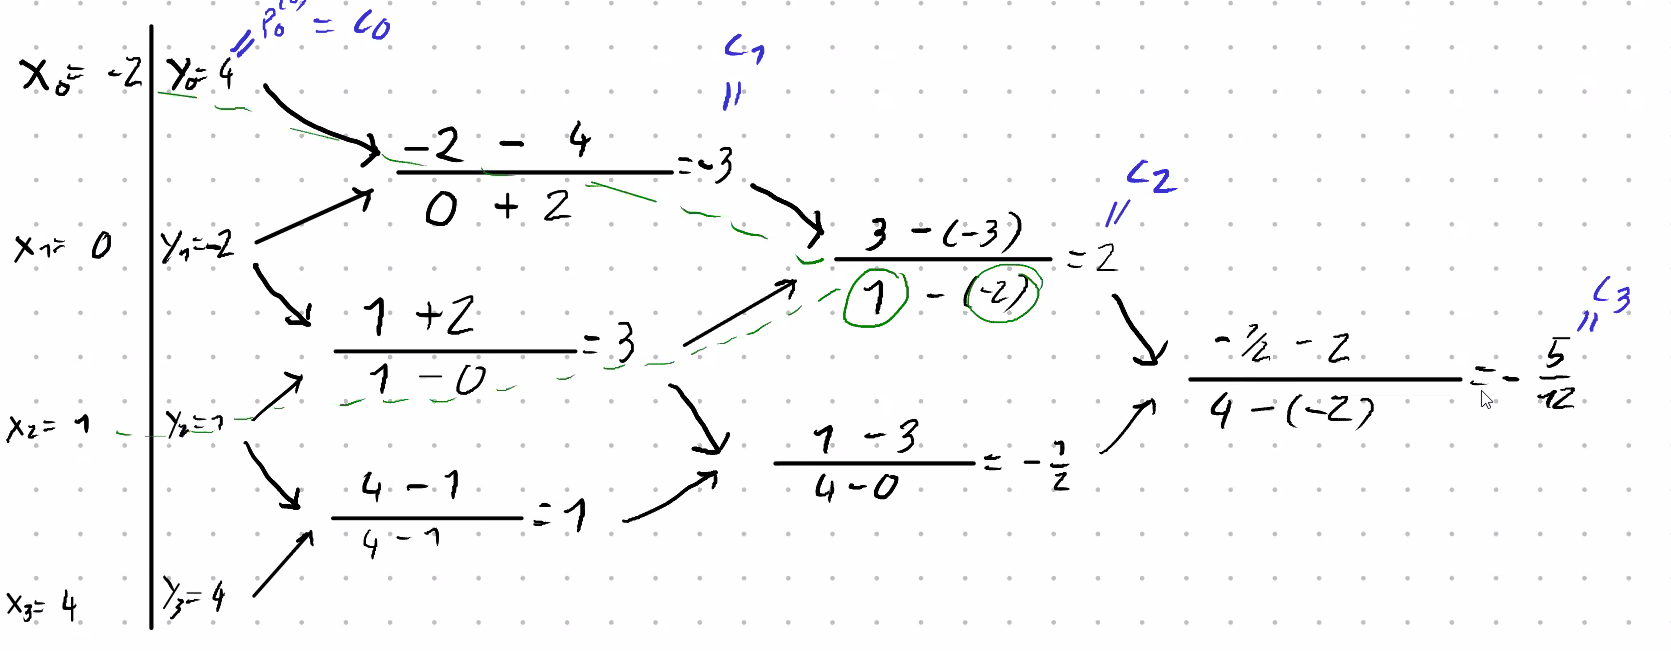
\includegraphics[width=256px]{Newton-Aitken-Nevill.png}\\
	Nebeinander liegende y's subtrahieren. für erstes nenner-x den Pfeilen nach unten folgen.\\
	Für zweites den Pfeilen nach oben.\\
	c) effizienter Auswertung von Polynomen\\
	Horner-Schema:\\
	$p(x)=4+(x+2)[-3 +2(x-5/12 x(x-1))]$\\
	wiederholen x ausklammern\\
	$p(x)=4+(x+2)[-3 +2x(1-5/12(x-1))]$\\
	\section{lokale Interpolation mit Catmul-Rom-interpolation}
	kleine Teilpolynome aneinanderketten.\\
	Stützstellen $\{(-3,-1),(-1,1),(1,2),(3,2)\}$
	Catmull-Rom ist Glatt in jedem Punkt (also stetig diff'bar)\\
	Zentrale Differenz allgemein
	\[y'_k=\frac{y_{k+1}-y_{k-1}}{x_{k+1}-x_{k-1}}\]
	Zentrale Differenz zwischen $(x_1,y_1)$ und $(x_3,y_3)$: $y_2'=\frac{2-(-1)}{1-(-3)}=\frac{3}{4}$ (wir haben eine equidistante Schrittweite 2)\\
	Zentrale Differenz zwischen $(x_4,y_4)$ und $(x_2,y_2)$ $y_3' = \frac{2-1}{3-(-1)} = \frac{1}{4}$\\
	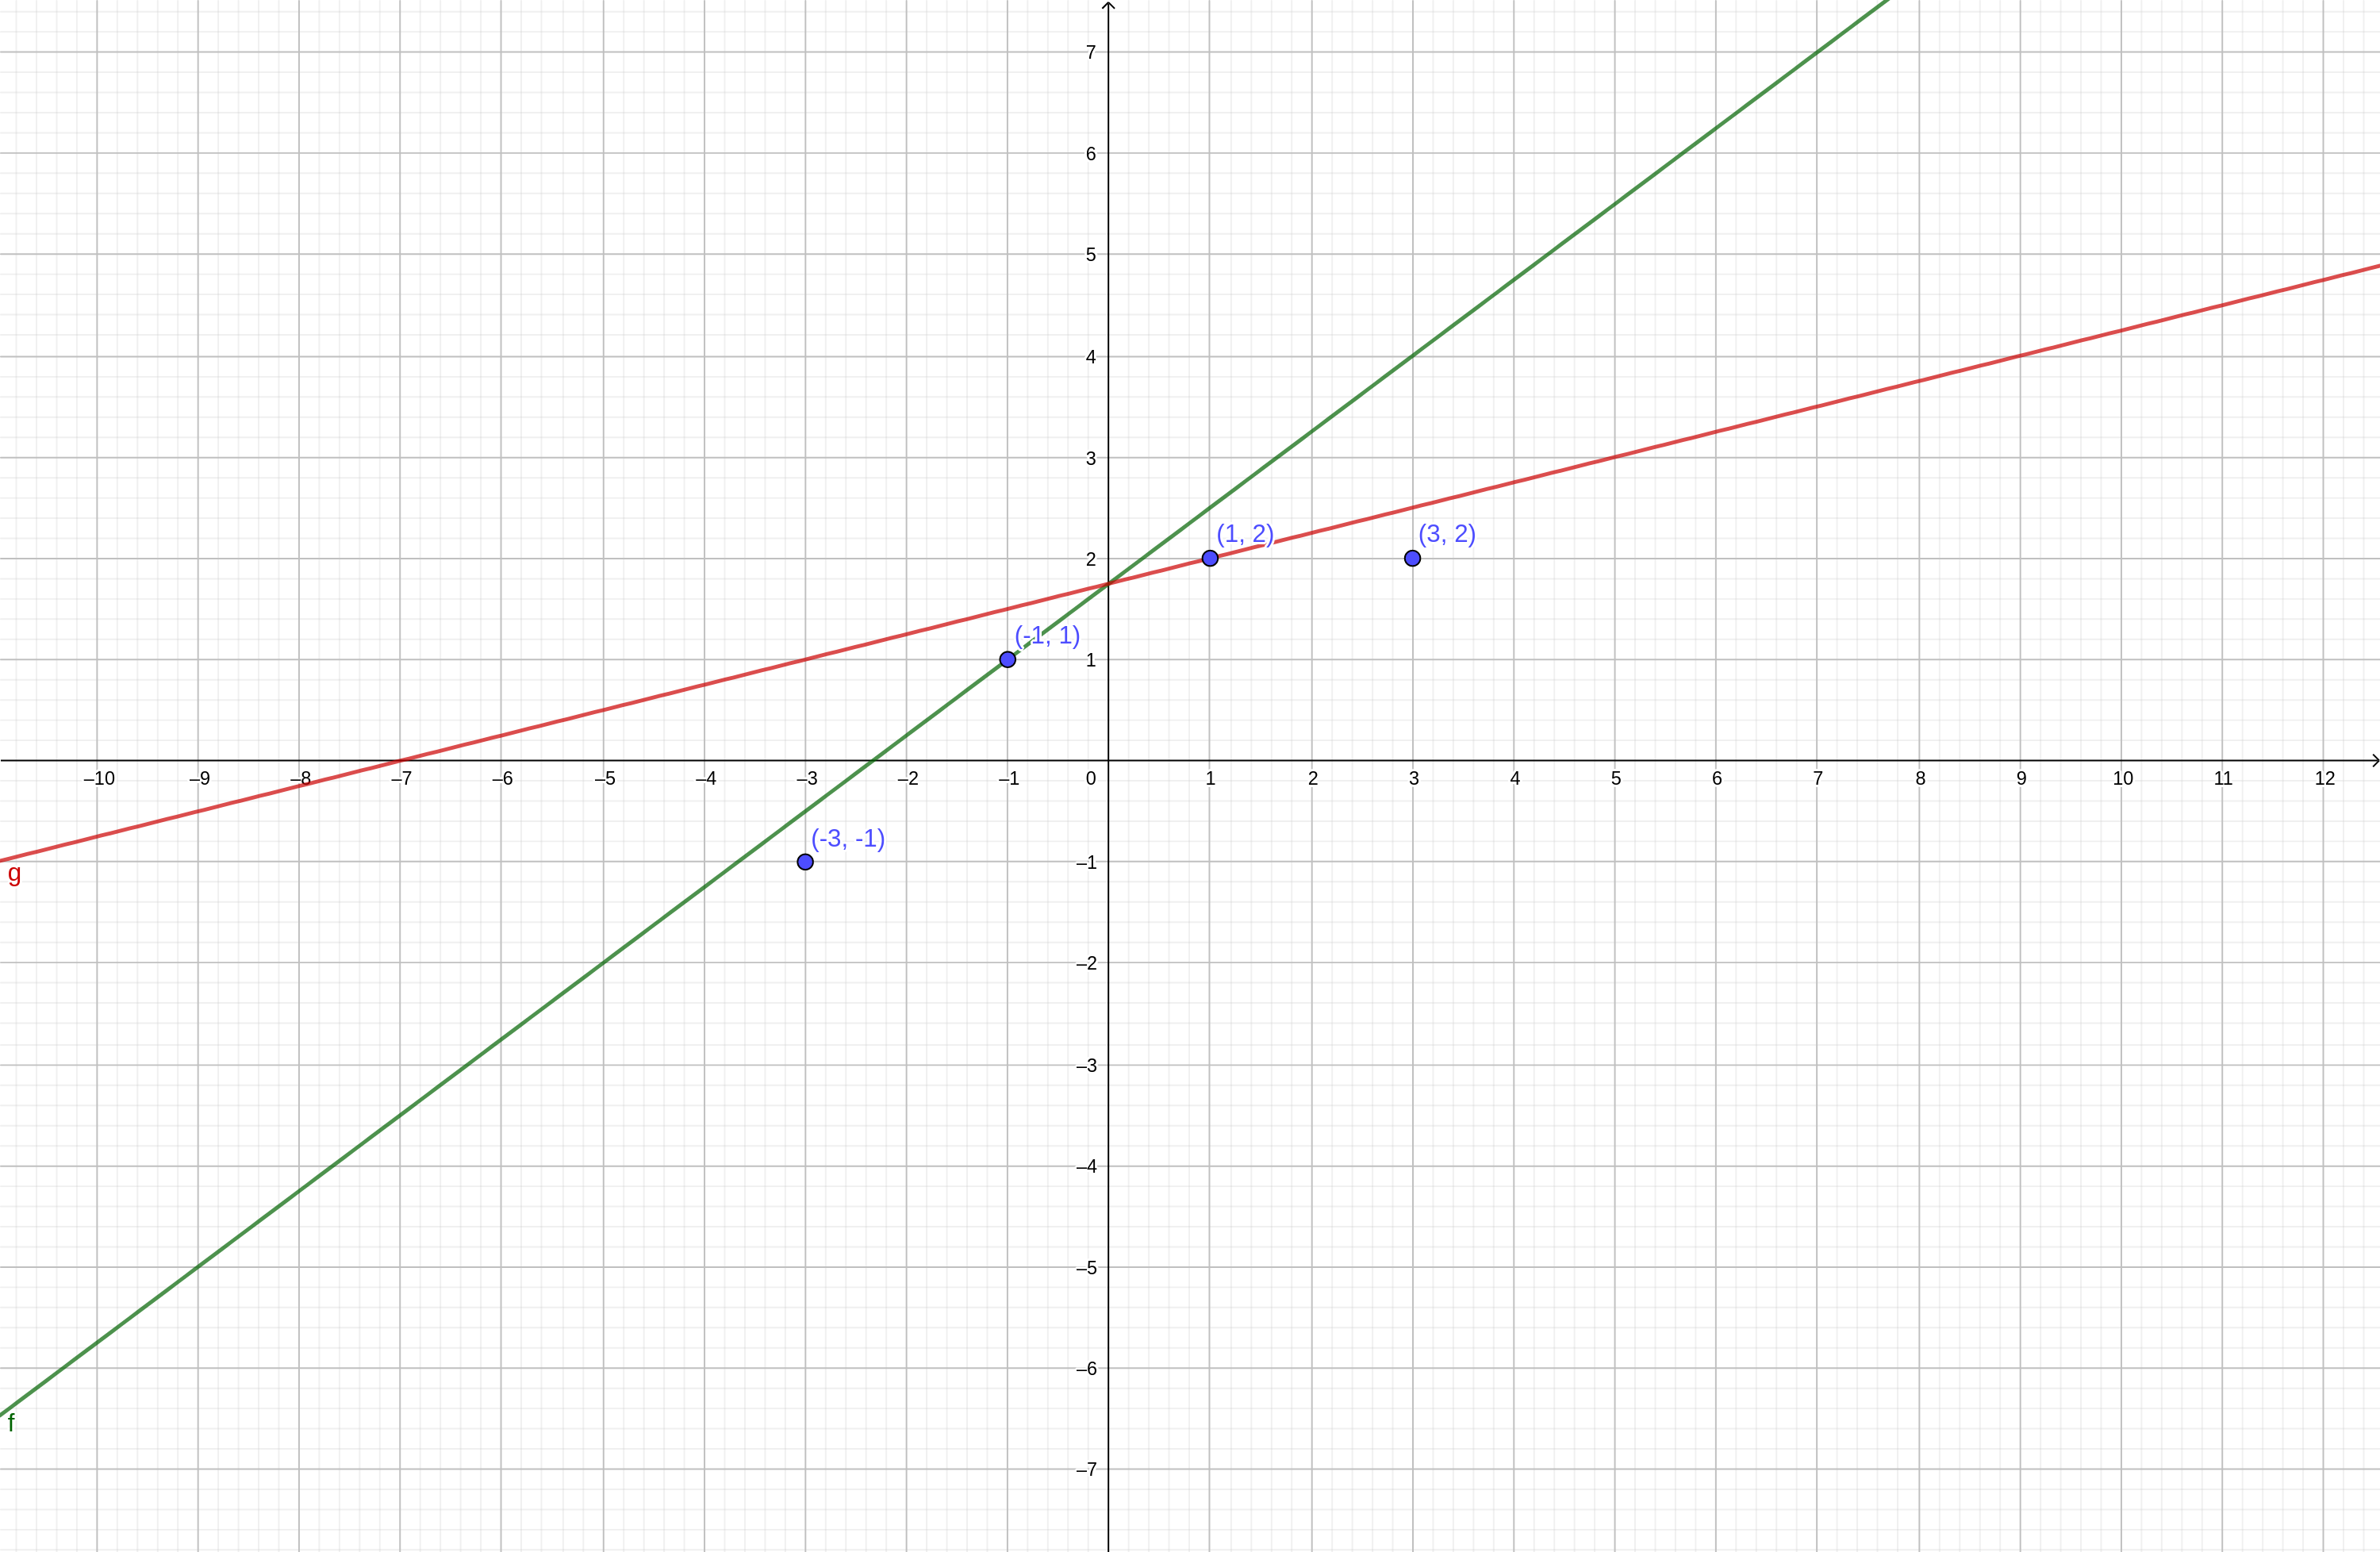
\includegraphics[width=256px]{Catmull-Rom.png}
\end{document}
